\documentclass[a4paper, 11pt]{article}
\usepackage{geometry}
\usepackage{url}
\usepackage{color}
\usepackage{booktabs}
\usepackage{tabularx}
\usepackage{tikz}
\usetikzlibrary{positioning,arrows.meta}


\linespread{1}

\geometry{a4paper,top=3cm,left=3cm,right=2.5cm,bottom=2cm}

\usepackage{hyperref}
\hypersetup{colorlinks,linkcolor=black,citecolor=blue}


\title{\textbf{Laboratory assignment} \\[1ex] \large \textbf{Component 4}}

\author{\textbf{Author: Ștefan-Lucian Grămadă}}

\begin{document}

\maketitle

\section{Related Work Summary}

This section summarises the literature approaches that address the same learning task and use the same data set. The task is to classify six activities of daily living from smartphone inertial signals: walking, walking upstairs, walking downstairs, sitting, standing and laying. The data set is the UCI Human Activity Recognition data set, referred to below as UCI HAR. The approaches are grouped into methods based on support vector machines, or SVMs, which work on the 561 engineered features, and deep learning methods, which work on the raw inertial signals. The approaches and their reported results are summarised in Tables~\ref{tab:approaches} and~\ref{tab:results}. Figure~\ref{fig:pipeline} shows the pipeline shared by the two groups of approaches.

\begin{figure}[ht]
\centering
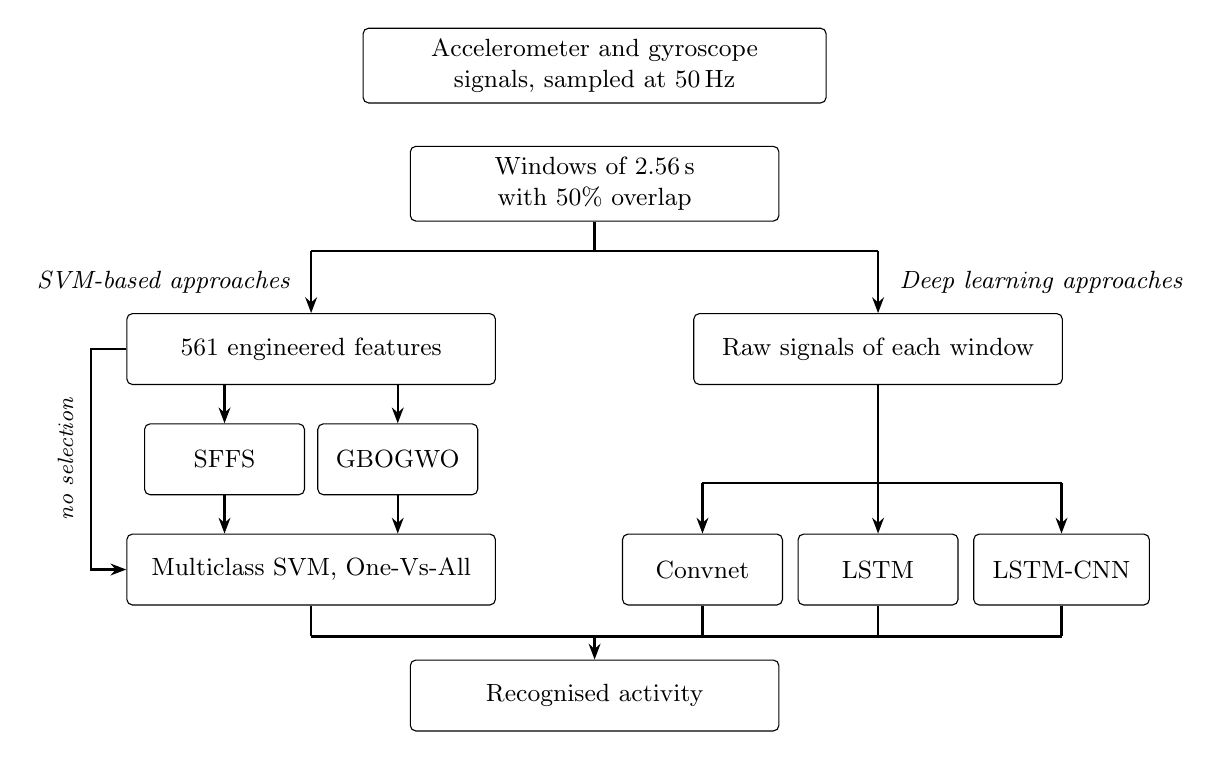
\begin{tikzpicture}[
  font=\small,
  box/.style={draw, rounded corners=2pt, align=center, text width=4.4cm, minimum height=0.9cm, inner sep=4pt, execute at begin node={\hyphenpenalty=10000}},
  sbox/.style={box, text width=1.75cm},
  arr/.style={-{Stealth[length=2mm]}, thick},
  lbl/.style={font=\small\itshape}
]
\node[box, text width=5.6cm] (sig) at (0,0) {Accelerometer and gyroscope signals, sampled at 50\,Hz};
\node[box] (win) at (0,-1.5) {Windows of 2.56\,s with 50\% overlap};
% SVM-based branch
\node[box] (feat) at (-3.6,-3.6) {561 engineered features};
\node[sbox] (sffs) at (-4.7,-5.0) {SFFS};
\node[sbox] (gbo) at (-2.5,-5.0) {GBOGWO};
\node[box] (svm) at (-3.6,-6.4) {Multiclass SVM, One-Vs-All};
% deep learning branch
\node[box] (raw) at (3.6,-3.6) {Raw signals of each window};
\node[sbox] (cnn) at (1.37,-6.4) {Convnet};
\node[sbox] (lstm) at (3.6,-6.4) {LSTM};
\node[sbox, text width=1.95cm] (lc) at (5.93,-6.4) {\mbox{LSTM-CNN}};
\node[box] (act) at (0,-8.0) {Recognised activity};
\node[lbl, anchor=east] at (-3.75,-2.75) {SVM-based approaches};
\node[lbl, anchor=west] at (3.75,-2.75) {Deep learning approaches};
% split after windowing
\draw[thick] (win.south) -- (0,-2.35);
\draw[thick] (-3.6,-2.35) -- (3.6,-2.35);
\draw[arr] (-3.6,-2.35) -- (feat.north);
\draw[arr] (3.6,-2.35) -- (raw.north);
% feature selection and bypass
\draw[arr] (feat.south -| sffs) -- (sffs.north);
\draw[arr] (feat.south -| gbo) -- (gbo.north);
\draw[arr] (sffs.south) -- (svm.north -| sffs);
\draw[arr] (gbo.south) -- (svm.north -| gbo);
\draw[arr] (feat.west) -- ++(-0.45,0) |- (svm.west);
\node[lbl, font=\footnotesize\itshape, rotate=90, anchor=south] at (-6.5,-5.0) {no selection};
% deep networks
\draw[thick] (raw.south) -- (3.6,-5.3);
\draw[thick] (1.37,-5.3) -- (5.93,-5.3);
\draw[arr] (1.37,-5.3) -- (cnn.north);
\draw[arr] (3.6,-5.3) -- (lstm.north);
\draw[arr] (5.93,-5.3) -- (lc.north);
% merge
\draw[thick] (svm.south) -- (-3.6,-7.25);
\draw[thick] (cnn.south) -- (1.37,-7.25);
\draw[thick] (lstm.south) -- (3.6,-7.25);
\draw[thick] (lc.south) -- (5.93,-7.25);
\draw[thick] (-3.6,-7.25) -- (5.93,-7.25);
\draw[arr] (0,-7.25) -- (act.north);
\end{tikzpicture}
\caption{Pipeline of the approaches evaluated on UCI HAR. The SVM-based approaches classify engineered features, while the deep learning approaches learn the features from the raw signals of each window.}
\label{fig:pipeline}
\end{figure}

\subsection{The UCI HAR data set and the original SVM baseline}

The data set was introduced by Anguita et al.~\cite{anguita2013}. Thirty volunteers performed the six activities while wearing a Samsung Galaxy S II smartphone on the waist. The accelerometer and the gyroscope of the phone were sampled at 50\,Hz. The signals were filtered, the acceleration was separated into a body component and a gravity component, and the signals were cut into windows of 2.56\,s with an overlap of 50\%. A total of 561 time and frequency domain features were computed for each window. The data were divided into a training set with 70\% of the data and a test set with the remaining 30\%.

As a reference result, the authors trained a multiclass SVM built from binary SVMs with the One-Vs-All strategy. They used Gaussian kernels and selected the hyperparameters by 10-fold cross-validation. The model reached an overall accuracy of 96\% on the 2947 test patterns. Laying was recognised perfectly, with a recall of 100\%. Sitting had the lowest recall, 88\%, because 57 sitting windows were classified as standing. The authors attribute this confusion to the position of the phone on the body.

An earlier work by the same group~\cite{anguita2012} proposed a hardware-friendly multiclass SVM, called MC-HF-SVM, for activity recognition on the phone itself. It replaces floating-point arithmetic with fixed-point arithmetic, which requires less memory, processor time and energy. The experiments used an earlier version of the data. It had the same 30 volunteers and six activities, but only 17 features computed from the accelerometer signals and 789 test samples. The standard floating-point multiclass SVM reached an accuracy of 89.3\%, and the MC-HF-SVM with 8 bits reached 89.0\%. The authors report that 6 bits are sufficient for a performance comparable to the floating-point model. Since the data differ from the public UCI HAR release, this result is not included in Table~\ref{tab:results}.

\subsection{SVM-based approaches with feature selection}

Later SVM-based works keep the engineered features but reduce their number before classification.

Ahmed et al.~\cite{ahmed2020} proposed a hybrid feature selection model, in which a filter step is followed by a wrapper step. The wrapper step uses sequential floating forward search, or SFFS~\cite{pudil1994}. The selected features are classified with a One-Vs-All multiclass SVM. The validation of the selected features is described with a linear kernel, chosen for its simplicity and computational efficiency, although the abstract mentions non-linear classifiers obtained with the kernel trick. The authors first used an extended version of the data set with 12 activities, which adds six postural transitions to the six basic activities. On this version, the selected features gave an average accuracy of 96.81\%, compared to 90.84\% without feature selection. On the six-activity UCI HAR data set, the same model reached an accuracy of 98.13\%.

Helmi et al.~\cite{helmi2021} proposed GBOGWO, a metaheuristic feature selection method. It combines the gradient-based optimizer, or GBO~\cite{ahmadianfar2020}, with operators of the grey wolf optimizer, or GWO~\cite{mirjalili2014}. Each candidate feature subset is evaluated by training a multiclass SVM. On UCI HAR, the method reduced the 561 features to 304 on average, a reduction of 45.8\%. It reached a mean accuracy of 98\% and a mean precision of 98.13\%. According to a Wilcoxon test, it outperformed the other optimizers in the comparison. The method was also evaluated on the WISDM data set.

\subsection{Deep learning approaches}

Deep learning approaches skip the manual feature engineering and learn features directly from the raw inertial signals of each window.

Ronao and Cho~\cite{ronao2016} proposed a deep convolutional neural network, or convnet, for smartphone-based activity recognition. The network exploits the temporally local dependency of the time series and learns increasingly complex features in its deeper layers. Its input consists of the raw triaxial accelerometer and gyroscope signals, that is six channels. The evaluation uses the standard split of UCI HAR, with 7352 training and 2947 test examples. The best convnet reached an accuracy of 94.79\% on the test set. When the fast Fourier transform of the signals was added to the input, the accuracy increased to 95.75\%. In the same comparison, an SVM on hand-crafted features reached 94.61\%. The convnet classified the moving activities almost perfectly, with an accuracy of 99.66\%, but the SVM performed better on the stationary activities.

Zhao et al.~\cite{zhao2018} proposed a deep residual bidirectional network built from long short-term memory cells, or LSTM cells. The bidirectional layers process the sequence in both time directions, and the residual connections between stacked layers help the gradients flow during training. Instead of the 561 features, the network uses only nine raw signals as input: the triaxial gravity acceleration, the triaxial body acceleration and the triaxial angular velocity. On UCI HAR, it reached an accuracy of 93.6\% and an F1 score of 93.5\%, compared to 90.8\% for a baseline LSTM. The network was also evaluated on the OPPORTUNITY data set.

Xia et al.~\cite{xia2020} proposed an LSTM-CNN architecture, in which the raw signals are fed to a two-layer LSTM followed by convolutional layers. A global average pooling layer replaces the fully connected layer to reduce the number of parameters, and a batch normalisation layer speeds up convergence. The model reached an overall accuracy of 95.78\% on UCI HAR, 95.85\% on WISDM and 92.63\% on OPPORTUNITY.

\subsection{Summary of the reported results}

Table~\ref{tab:approaches} summarises the approaches evaluated on UCI HAR with six activities, and Table~\ref{tab:results} summarises their reported results. The values are taken as reported by the authors. Since the authors used different evaluation settings, the values are only approximately comparable.

\begin{table}[ht]
\centering
\small
\renewcommand{\arraystretch}{1.4}
\begin{tabularx}{\textwidth}{@{}l >{\raggedright\arraybackslash}X l@{}}
\toprule
\textbf{Work} & \textbf{Approach} & \textbf{Input} \\
\midrule
Anguita et al.~\cite{anguita2013} & Gaussian SVM, One-Vs-All & 561 features \\
\midrule
Ahmed et al.~\cite{ahmed2020} & SFFS feature selection + SVM, One-Vs-All & selected features \\
\midrule
Helmi et al.~\cite{helmi2021} & GBOGWO feature selection + multiclass SVM & 304 of 561 features \\
\midrule
Ronao and Cho~\cite{ronao2016} & Convnet & 6 raw signals \\
\midrule
Ronao and Cho~\cite{ronao2016} & Convnet with FFT input & 6 raw signals + FFT \\
\midrule
Zhao et al.~\cite{zhao2018} & Deep residual bidirectional LSTM & 9 raw signals \\
\midrule
Xia et al.~\cite{xia2020} & LSTM followed by CNN & raw signals \\
\bottomrule
\end{tabularx}
\caption{Approaches evaluated on the UCI HAR data set with six activities.}
\label{tab:approaches}
\end{table}

\begin{table}[ht]
\centering
\small
\renewcommand{\arraystretch}{1.4}
\begin{tabular}{@{}lll@{}}
\toprule
\textbf{Work} & \textbf{Accuracy} & \textbf{Other reported metrics} \\
\midrule
Anguita et al.~\cite{anguita2013} & 96\% & -- \\
\midrule
Ahmed et al.~\cite{ahmed2020} & 98.13\% & -- \\
\midrule
Helmi et al.~\cite{helmi2021} & 98\% & precision 98.13\% \\
\midrule
Ronao and Cho~\cite{ronao2016}, convnet & 94.79\% & -- \\
\midrule
Ronao and Cho~\cite{ronao2016}, convnet with FFT input & 95.75\% & -- \\
\midrule
Zhao et al.~\cite{zhao2018} & 93.6\% & F1 score 93.5\% \\
\midrule
Xia et al.~\cite{xia2020} & 95.78\% & -- \\
\bottomrule
\end{tabular}
\caption{Results reported in the literature on the UCI HAR data set with six activities.}
\label{tab:results}
\end{table}

The results show that SVMs on the engineered features remain competitive with deep learning models on this data set. The original SVM baseline, with 96\%, is above the reported results of all three deep learning models, and the two SVM-based works with feature selection report the highest values, of about 98\%. Deep learning models avoid the manual feature engineering, but they have to learn the features from the raw signals. In the works that discuss per-class results~\cite{anguita2013,helmi2021,ronao2016}, the main difficulty is the separation of the stationary activities, especially sitting and standing.

The model used in this project is closest to the SVM-based works. It is a multiclass SVM with the One-Vs-Rest strategy trained on the 561 features, but with a linear kernel, while the original baseline~\cite{anguita2013} uses Gaussian kernels. Unlike these works, it is implemented from scratch, trained with Pegasos~\cite{Shalev-Shwartz2011} and evaluated by cross-validation instead of a single train/test split. These differences will be taken into account when the obtained results are compared to the literature in Component~5.

\bibliographystyle{alpha}
\bibliography{biblio}

\end{document}
